\section{Descrição de Software}

O pacote de trabalho de Planejamento e Gerenciamento foi modelado utilizando a notação BPMN, conforme ilustrado na Figura~\ref{fig_bpmn}. A utilização do BPMN permite representar de forma clara e padronizada os processos do projeto, facilitando a compreensão, a análise e a comunicação entre os envolvidos. Por meio desse modelo, é possível visualizar as atividades, os responsáveis, os fluxos de informações e as dependências, contribuindo para uma gestão mais eficiente e alinhada aos objetivos do projeto.

\begin{figure}[H]
\centering
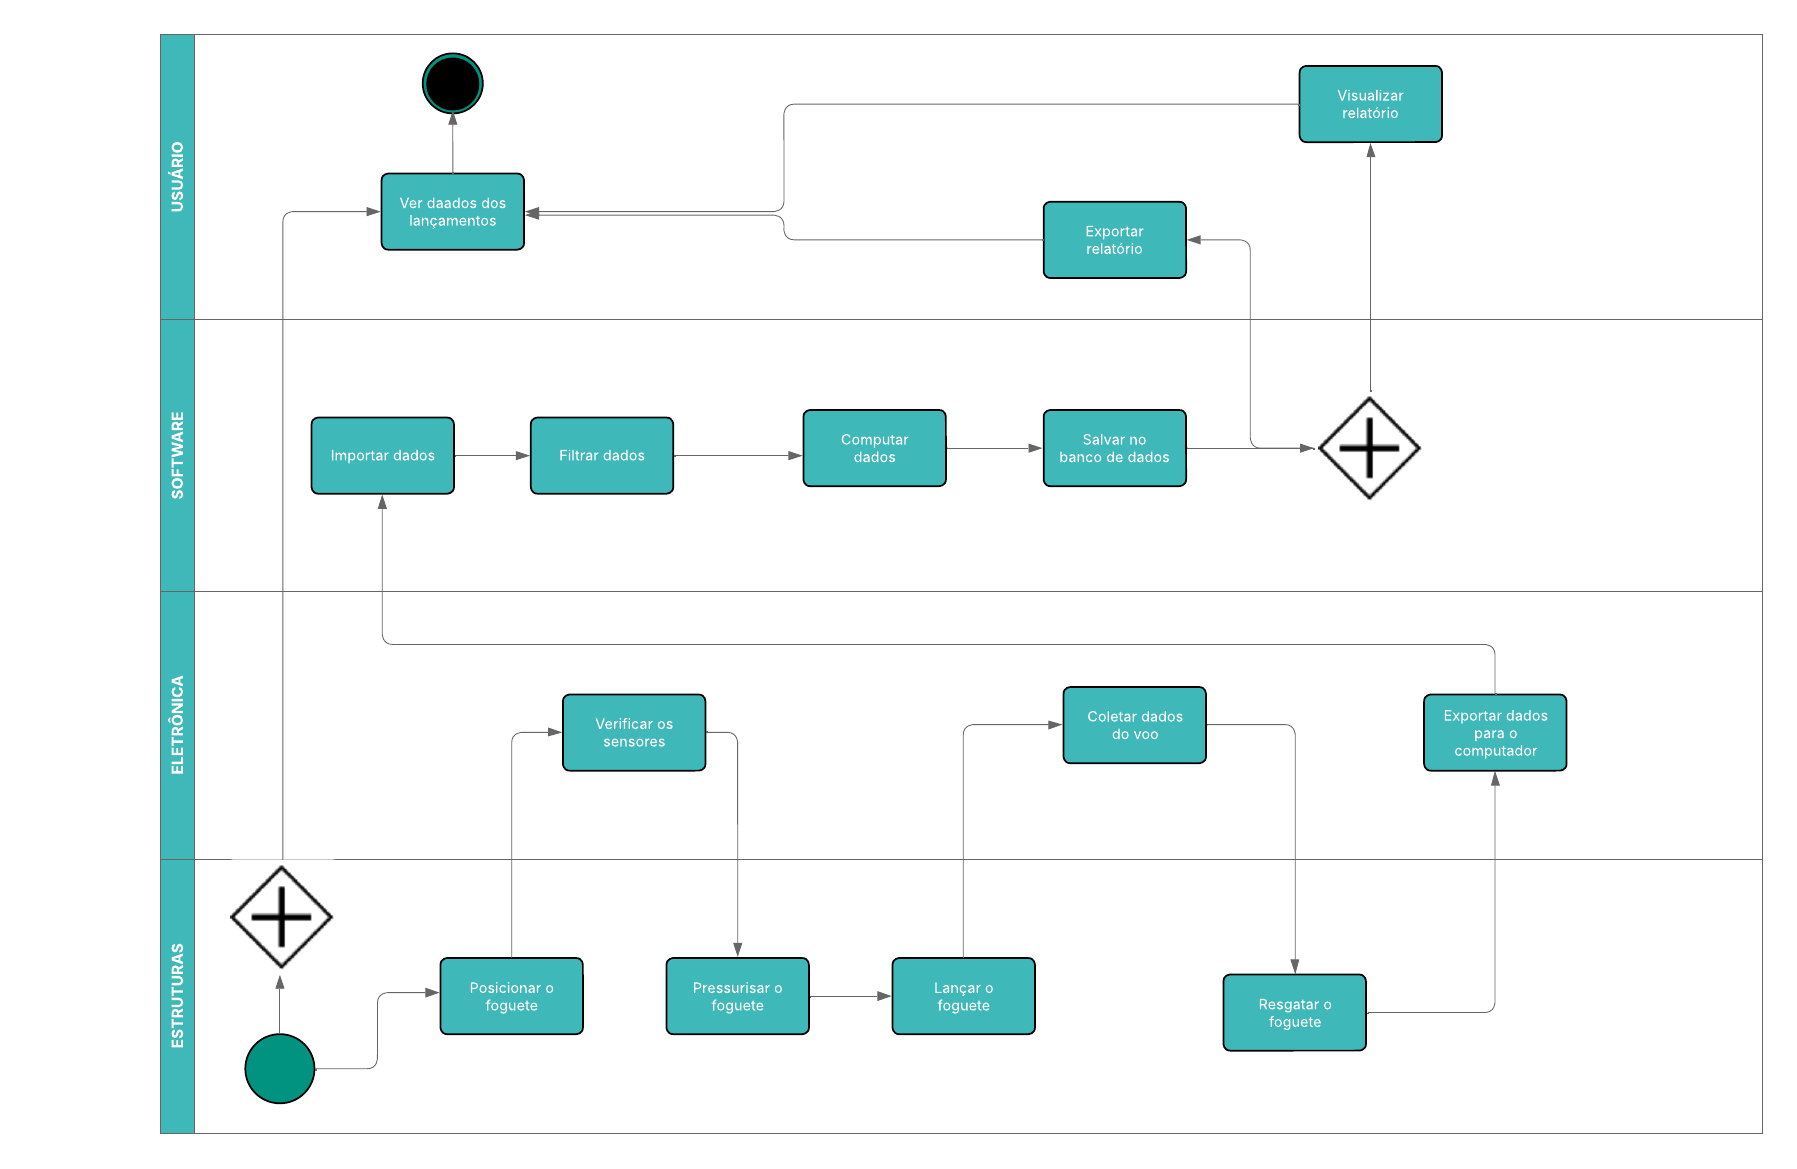
\includegraphics[width=15cm]{figuras/bpmn.png}
\caption{BPMN}
\label{fig_bpmn}
\end{figure}

% -------------------------------------------------------------
% MOSCOW
% -------------------------------------------------------------

\begin{samepage}
O pacote MOSCOW é uma técnica de priorização de requisitos que classifica as funcionalidades em quatro categorias: Must have (deve ter), Should have (deveria ter), Could have (poderia ter) e Won't have this time (não terá desta vez). Essa abordagem ajuda a focar no que é essencial para o sucesso do projeto, garantindo que os recursos sejam alocados de forma eficiente. A Figura \ref{tab:requisitos_projeto} ilustra a aplicação dessa técnica no contexto do projeto.

\begin{landscape}

\begin{figure}[H]
\centering
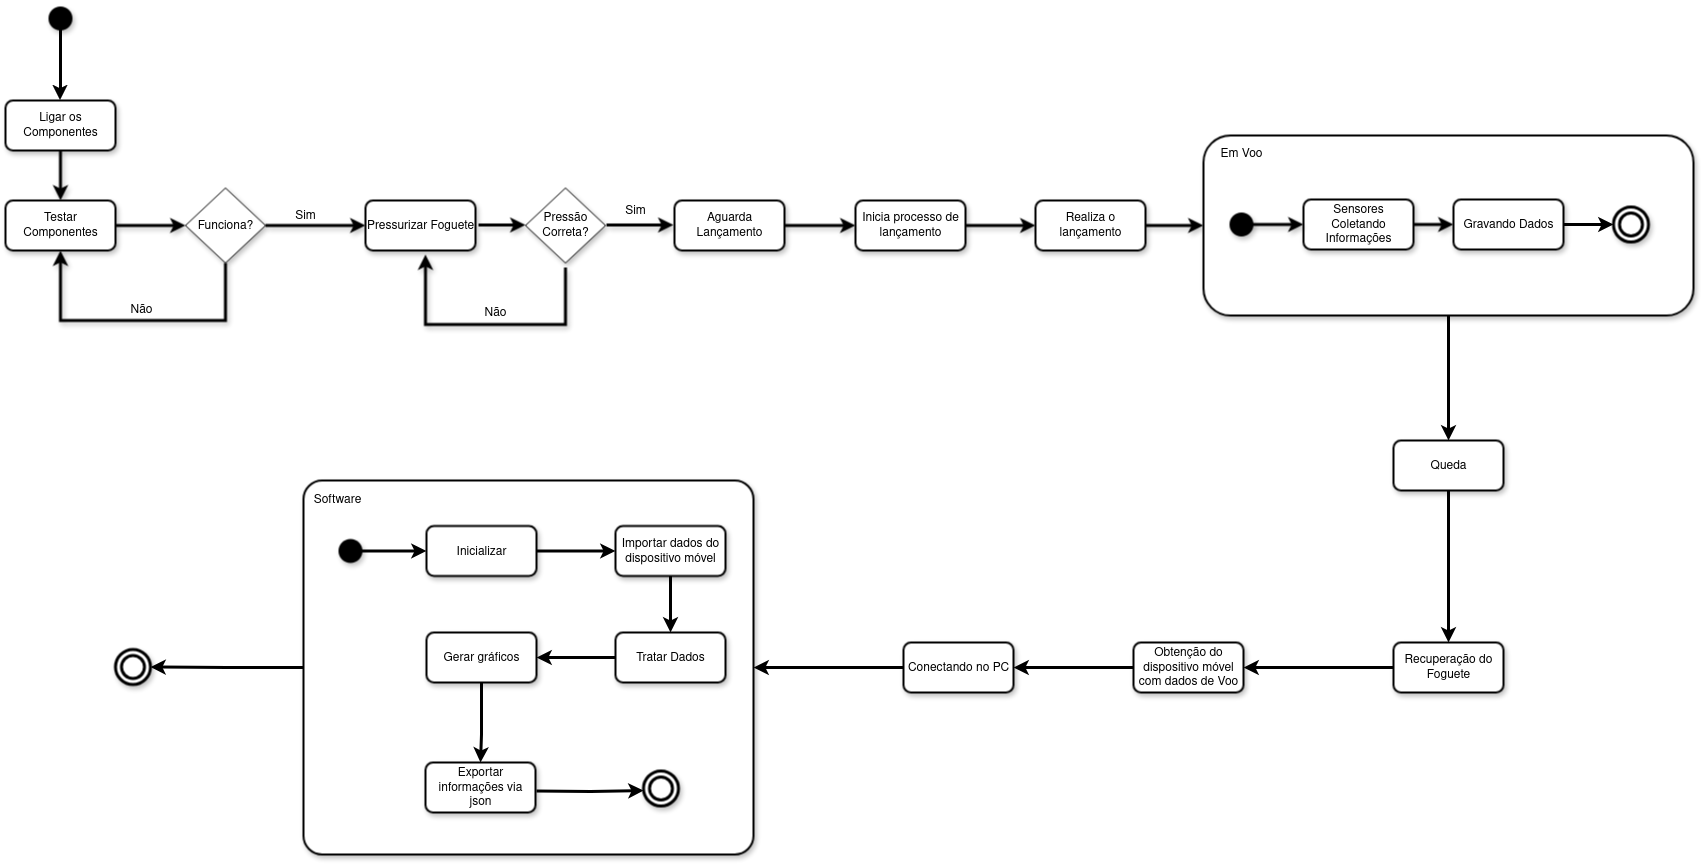
\includegraphics[width=\linewidth,keepaspectratio]{figuras/diagrama_de_estados.png}
\caption{Diagrama de Estados}
\label{fig_diagrama_estados}
\end{figure}

\end{landscape}


\begin{table}[H]
\centering
\scriptsize
\setlength{\tabcolsep}{4pt}
\caption{Tabela de Requisitos do Projeto}
\begin{tabular}{|l|p{8cm}|l|}
\hline
Id. & Descição & Prioridade \\
\hline
RQ01 & Importar dados de voo em JSON de dispositivo externo & Must have \\
\hline
RQ02 & Exibir gráfico de velocidade vertical vs. tempo. & Must have \\
\hline
RQ03 & Exibir gráfico de aceleração vertical vs. tempo. & Must have \\
\hline
RQ04 & Exibir gráfico de dispersão da trajetória no plano X e Y. & Must have \\
\hline
RQ05 & Exibir gráfico de altitude vs. tempo. & Must have \\
\hline
RQ06 & Exibir valores máximos e mínimos de aceleração, velocidade e ângulo. & Should have \\
\hline
RQ07 & Exibir tempo de execução e intervalos de amostragem. & Should have \\
\hline
RQ08 & Exportar dados do voo em JSON. & Must have \\
\hline
RQ09 & Importar arquivos JSON para comparação e simulação. & Must have \\
\hline
RQ10 & Aplicar filtro de média móvel nos dados dos sensores. & Should have \\
\hline
RQ11 & Inicializar o sistema de medição e sinalizar prontidão para o lançamento. & Must Have \\
\hline
RQ12 & Aplicar filtro de média móvel nos dados dos sensores. & Must Have \\
\hline
RQ13 & O mecanismo de lançamento deve permitir disparo seguro por tração de corda a pelo menos 5 metros. & Must Have \\
\hline
RQ14 & A plataforma de lançamento deve manter o foguete estável até o momento da liberação manual. & Must Have \\
\hline
\end{tabular}
\label{tab:requisitos_projeto}
\end{table}

\end{samepage}


% -------------------------------------------------------------
% REQUISITOS NÃO-FUNCIONAIS
% -------------------------------------------------------------

\begin{samepage}
Os requisitos não-funcionais são critérios que definem a qualidade e as restrições do sistema, como desempenho, segurança, usabilidade e portabilidade. Eles são essenciais para garantir que o sistema atenda às expectativas dos usuários e funcione de maneira eficiente em diferentes ambientes. A Tabela \ref{tab:requisitos_nao_funcionais} apresenta os requisitos não-funcionais identificados para o projeto.

\begin{table}[H]
\centering
\scriptsize
\setlength{\tabcolsep}{4pt}
\caption{Requisitos Não-Funcionais}
\begin{tabular}{|l|p{11cm}|}
\hline
Id. & Descrição \\
\hline
RNF01 & Os dados dos lançamentos devem ser armazenados localmente de forma que não possam ser corrompidos em caso de desligamento inesperado. \\
\hline
RNF02 & O software deve validar a integridade dos arquivos JSON antes de processar os dados. \\
\hline
RNF03 & O software deve ser multiplataforma, funcionando em pelo menos Windows, Linux e MacOS. \\
\hline
RNF04 & Não deve depender de conexão com internet para funcionar. \\
\hline
RNF05 & A geração de relatórios e gráficos não deve exceder 3 segundos para arquivos de até 100 linhas de dados do lançamento. \\
\hline
RNF06 & A interface gráfica (GUI) deve ser intuitiva, com botões claros para importar dados, gerar gráficos e acessar os lançamentos anteriores. \\
\hline
RNF07 & A interface de linha de comando (CLI – Command Line Interface) deve oferecer comandos simples para uso técnico ou automatizado. \\
\hline
\end{tabular}
\label{tab:requisitos_nao_funcionais}
\end{table}
\end{samepage}

% -------------------------------------------------------------
% CASOS DE USO
% -------------------------------------------------------------

\begin{samepage}

O pacote de Casos de Uso é uma técnica de modelagem que descreve as interações entre os usuários (atores) e o sistema, detalhando como os requisitos funcionais serão atendidos. Os casos de uso ajudam a identificar as funcionalidades essenciais do sistema e a garantir que todas as partes interessadas tenham uma compreensão clara dos objetivos do projeto. A Figura \ref{fig_casos_de_uso} apresenta um exemplo de diagrama de casos de uso utilizado no projeto.
\begin{figure}[H]
	\centering
	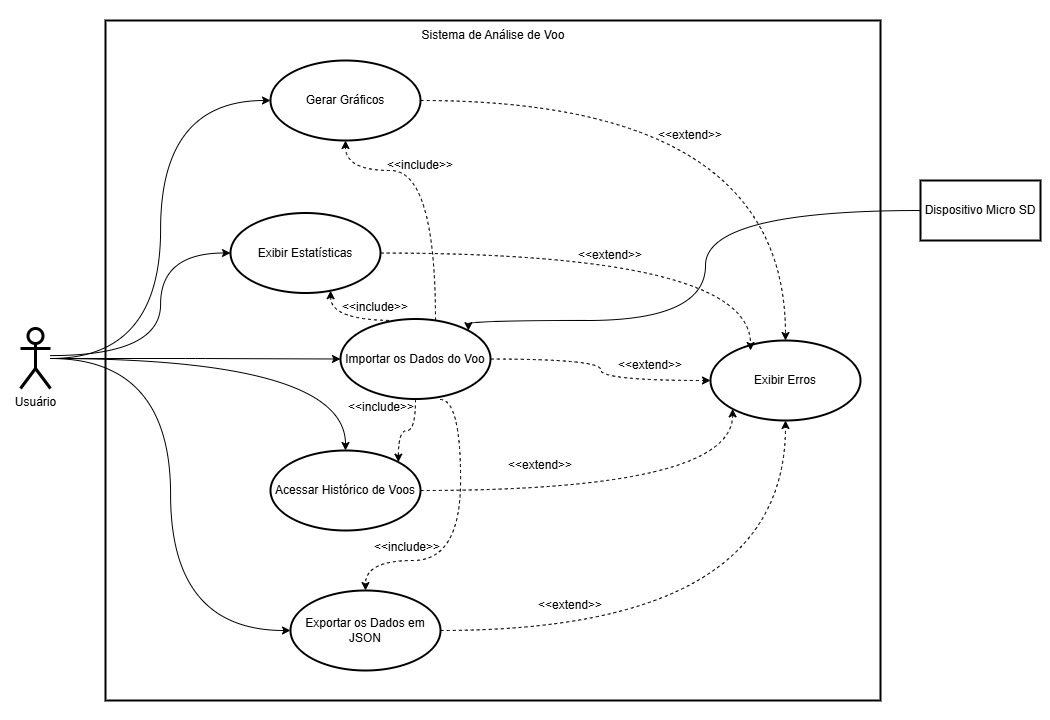
\includegraphics[width=15cm]{figuras/caso_de_uso.png}
	\caption{Casos de Uso}
	\label{fig_casos_de_uso}
\end{figure}
\end{samepage}

% -------------------------------------------------------------
% DIAGRAMA DE ENTIDADE-RELACIONAMENTO
% -------------------------------------------------------------

\begin{samepage}

O Diagrama de Entidade-Relacionamento (DER) é uma técnica de modelagem de dados que representa as entidades do sistema e os relacionamentos entre elas. É fundamental para a construção do banco de dados e para garantir que os dados sejam organizados de forma eficiente. A Figura \ref{fig_der} ilustra um exemplo de DER utilizado no projeto.

\begin{figure}[H]
	\centering
	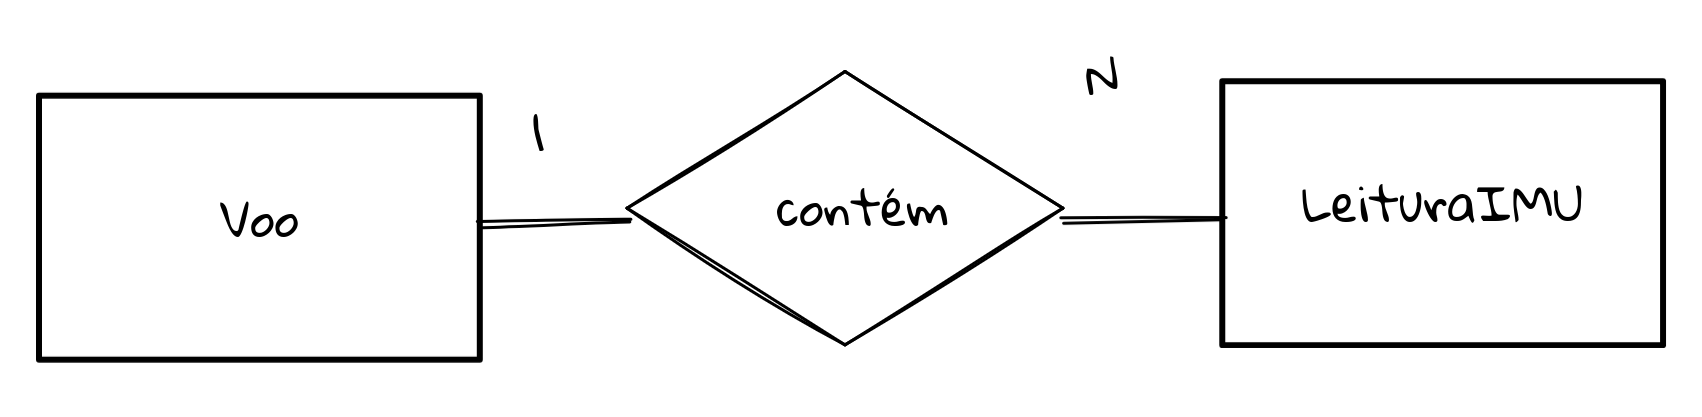
\includegraphics[width=15cm]{figuras/der.png}
	\caption{Diagrama de Entidade-Relacionamento}
	\label{fig_der}
\end{figure}

Após isso, podemos modelar os atributos de cada entidade, conforme os dados que receberemos da ERP32, que calculará movimentos de unidade de medição inercial pelo sensor de 6 eixos, como o acelerômetro e o giroscópio. A Figura \ref{fig_atributos} apresenta um exemplo de atributos modelados para as entidades do sistema.

\begin{figure}[H]
	\centering
	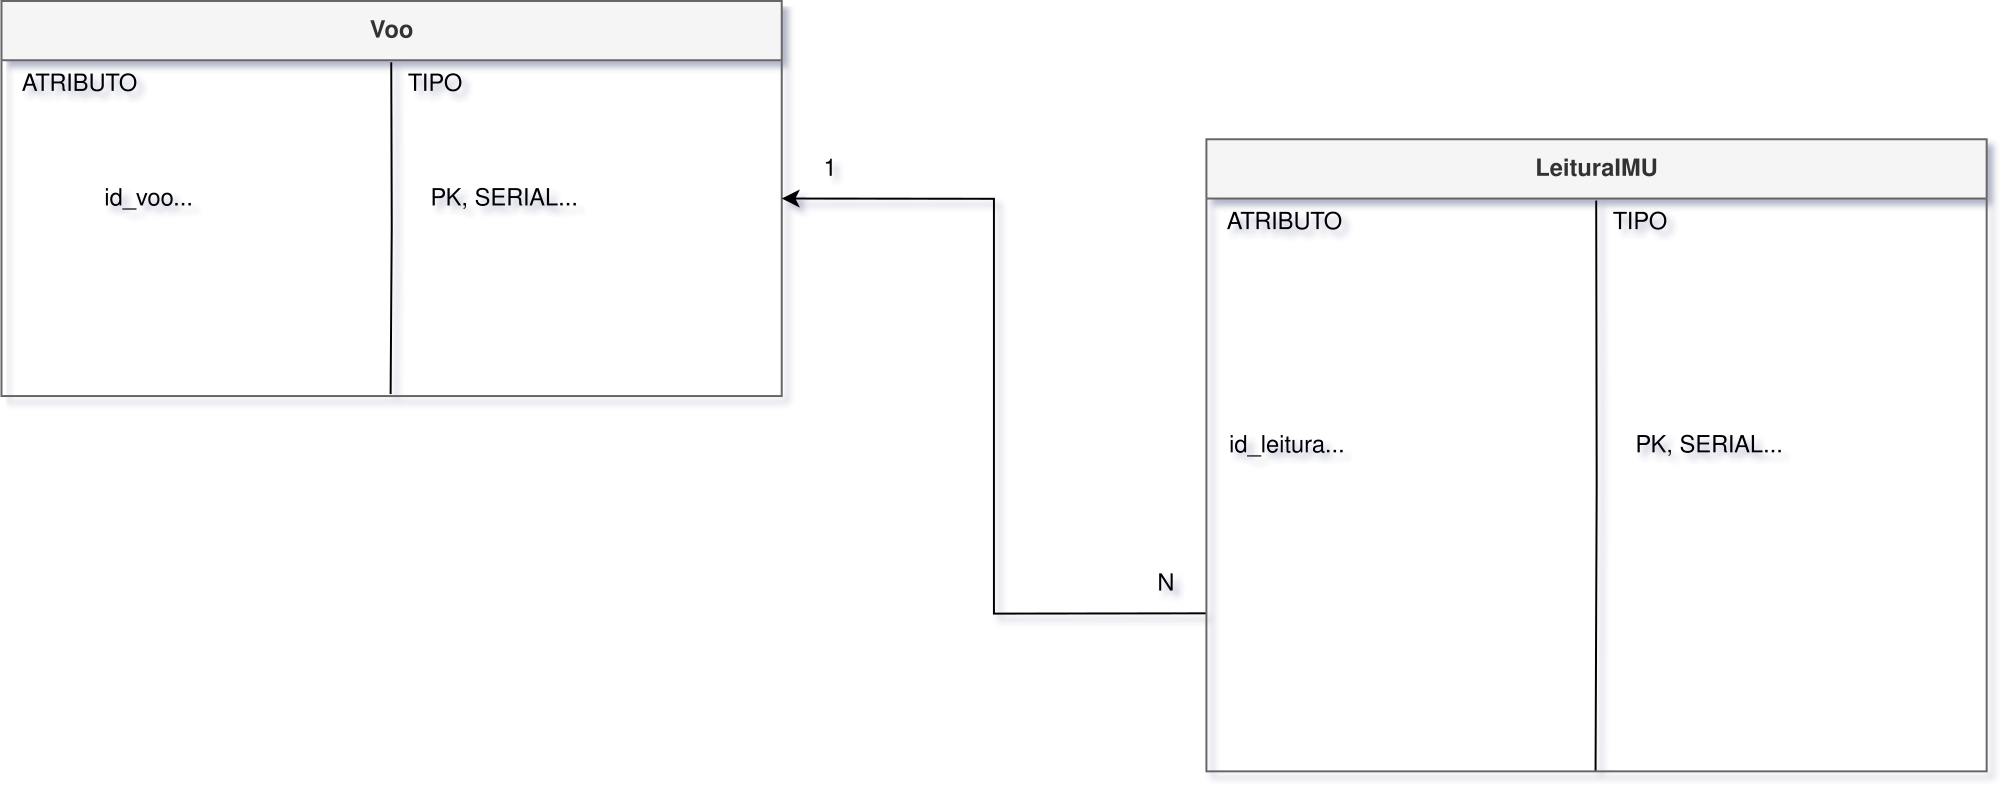
\includegraphics[width=15cm]{figuras/atributos.png}
	\caption{Atributos das Entidades}
	\label{fig_atributos}
\end{figure}

\end{samepage}

% -------------------------------------------------------------
% ARQUITETURA DO SOFTWARE
% -------------------------------------------------------------

\begin{samepage}

O padrão arquitetural escolhido é o Monolítico, por se tratar de um sistema simples, com poucos módulos e baixa complexidade. A adoção de uma arquitetura mais robusta, como microsserviços, não se justifica neste contexto, uma vez que todo o processamento ocorre localmente e o software não possui dependências distribuídas. 

A arquitetura monolítica permite concentrar todas as funcionalidades como leitura de dados, processamento, geração de relatórios e apresentação dos resultados em um único sistema, facilitando o desenvolvimento, testes e manutenção dentro dos requisitos do projeto, como visto na Figura \ref{fig_arquitetura}.

\begin{figure}[H]
	\centering
	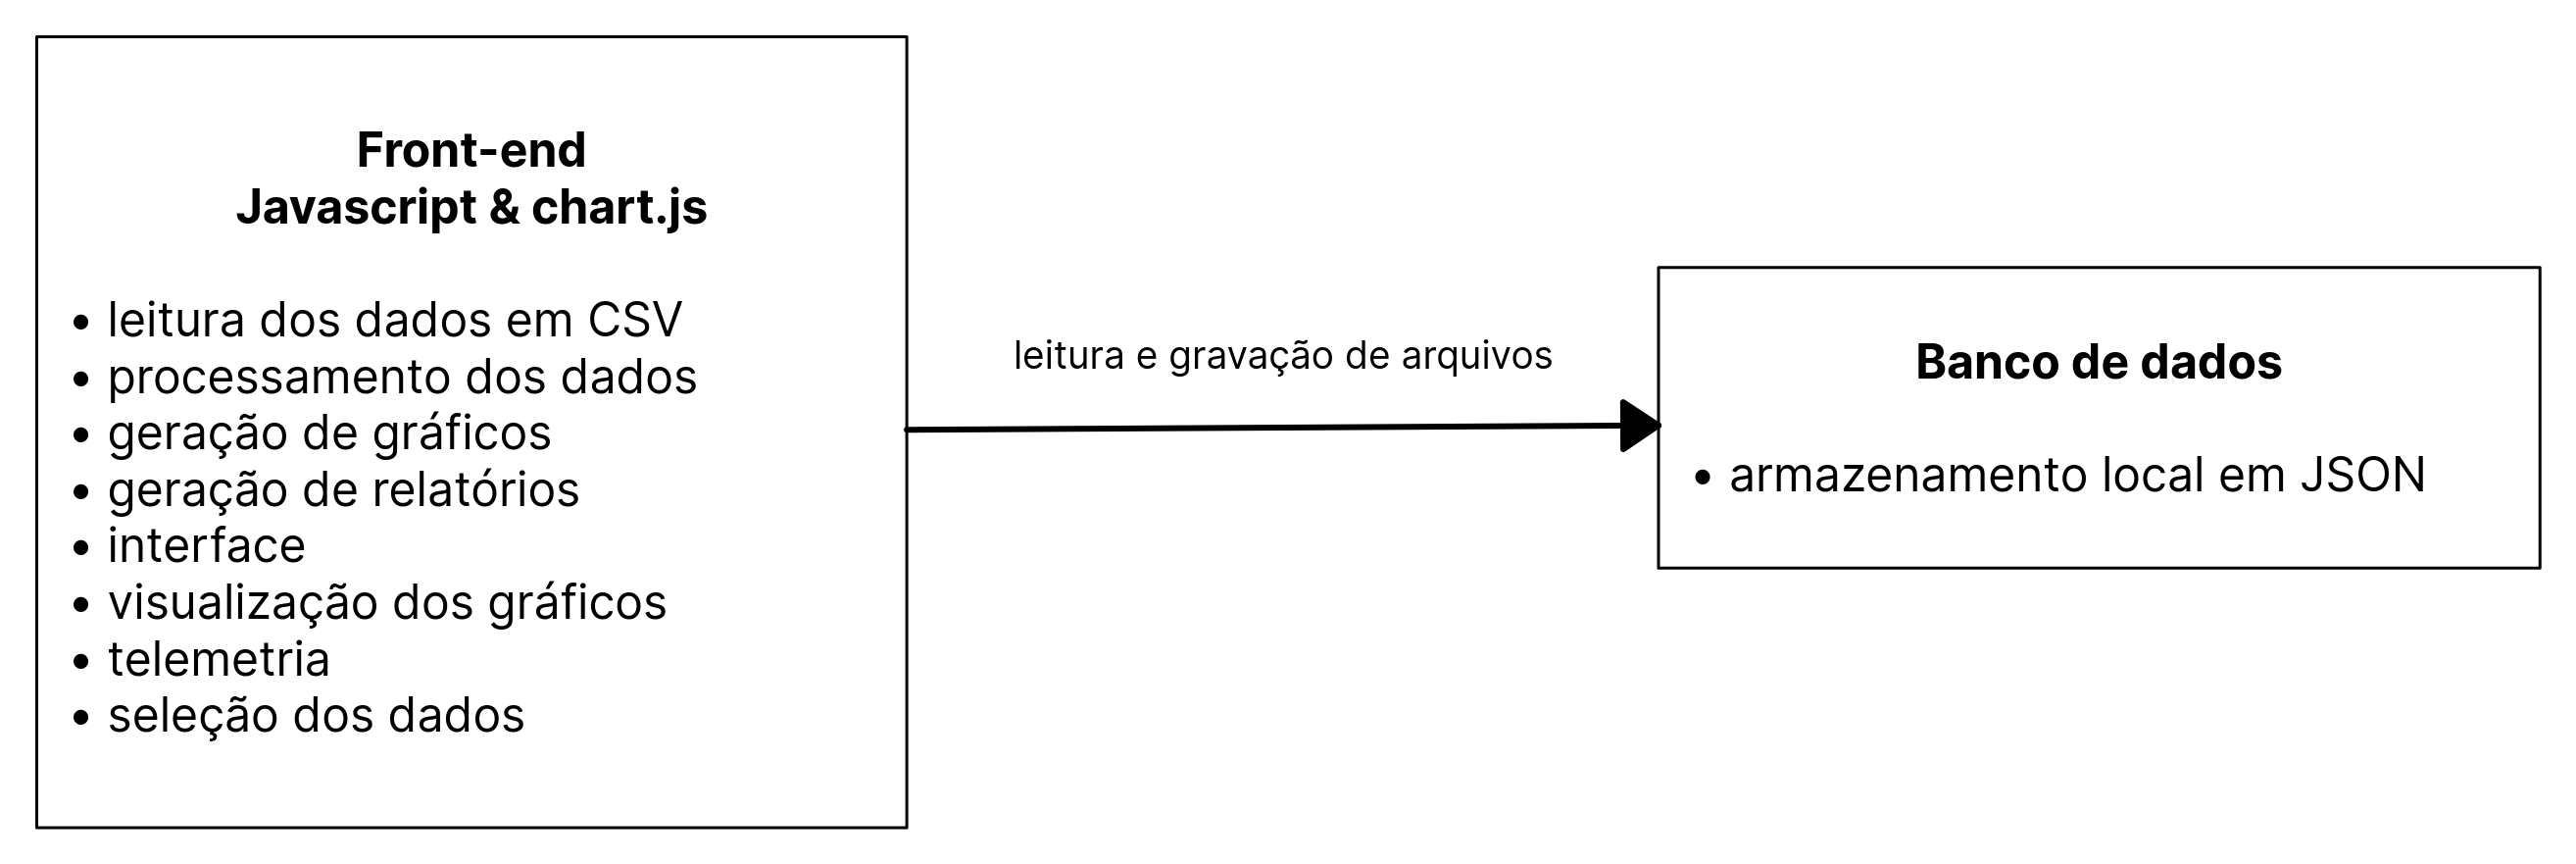
\includegraphics[width=0.75\textwidth,height=0.5\textheight,keepaspectratio]{figuras/arquitetura2.png}
	\caption{Arquitetura do Software}
	\label{fig_arquitetura}
\end{figure}

As linguagens de programação escolhidas para o desenvolvimento do software são Python e JavaScript, cada uma com suas responsabilidades específicas dentro do sistema.

Python foi responsável primariamente pelo desenvolvimento de uma interface de linha de comando (CLI). Utilizado para processamento dos dados, geração de relatórios, análises estatísticas e manipulação dos arquivos JSON até a segunda entrega. Utilizamos as bibliotecas Pandas para manipulação e análise de dados. NumPy para cálculos matemáticos e operações com arrays. E Matplotlib para criação de gráficos e visualizações dos dados.

JavaScript então foi utilizado no desenvolvimento do frontend (GUI), através da biblioteca Chart.JS, para então cumprir com as responsabilidades do CLI, e apresentando visualmente os dados dos lançamentos de forma interativa e amigável.

Neste projeto, não foi utilizado um banco de dados tradicional. Os dados dos lançamentos são armazenados localmente em arquivos JSON, por se tratar de uma solução leve, simples e suficiente para o volume de dados do projeto. Cada arquivo JSON conterá os dados de um lançamento específico, organizados de forma que possam ser facilmente acessados tanto pela CLI quanto pela interface gráfica.

\end{samepage}

% -------------------------------------------------------------
% PROTÓTIPO
% -------------------------------------------------------------

\begin{samepage}

O protótipo do software foi desenvolvido utilizando a ferramenta Figma, que permite criar interfaces interativas e de alta fidelidade. O protótipo inclui telas para importação de dados, visualização de gráficos, relatórios e histórico de lançamentos. Ele pode ser acessado em \href{https://www.figma.com/proto/hpceGFGo6mcwMjRJsKIyG7/Foguete-D-agua?node-id=19-2848&p=f&t=BINV4uEIBSLAGqsi-1&scaling=min-zoom&content-scaling=fixed&page-id=0%3A1&starting-point-node-id=19%3A2848}{neste endereço}.

\end{samepage}

% -------------------------------------------------------------
% MODIFICAR PARA EXPLICART OS TESTES DO PROJETO	
% -------------------------------------------------------------

\begin{samepage}

A principal mudança nos testes foi a especificação e detalhamento dos mesmos. Todos os casos de teste foram migrados do relatório para uma planilha no Microsoft Excel Online, como disponibilizado anteriormente, facilitando a visualização geral, o acompanhamento da execução e a atualização dos status de cada teste em tempo real por todos os membros da equipe. Ela pode ser completamente acessada em
%\url{https://unbbr.sharepoint.com/:x:/s/PI1-Grupo2330/EY-ZE1arh2RGgJju4ij_Er4BGhCN5S1qYQiIwdHMMRtLBg?e=fs9Vxi}
\href{https://unbbr.sharepoint.com/:x:/s/PI1-Grupo2330/EY-ZE1arh2RGgJju4ij_Er4BGhCN5S1qYQiIwdHMMRtLBg?e=fs9Vxi}{planilha de testes do grupo 2}.

% Para o caso de teste CT01, que envolve a importação de um arquivo JSON válido, foi adicionado um exemplo de arquivo JSON com dados reais do foguete. Esse arquivo contém informações como id do voo, tempo, aceleração e velocidade, permitindo uma validação mais precisa do processo de importação. No mesmo contexto, ao CT02 foi adicionado um arquivo JSON com campos ausentes, como id de leitura e tempo, para testar a robustez do sistema em lidar com dados incompletos. O CT03 foi modificado para incluir um arquivo JSON com formato inválido, como strings onde se esperavam números, para verificar a capacidade do sistema de identificar e reportar erros de formatação.

\subsection{Testes}

Aos testes CT01, CT02, CT03, CT08, CT11, CT13, CT14, CT15, CT16 foram adicionados os dados de arquivo necessário para realização do teste, a estrutura dos dados de entrada, especificação de resultados esperados e, para os que possui mensagens, as de sucesso e erro foram definidas. Para o teste de responsividade (CT05) foram definidos os tamanhos da tela para responsividade. 

Na parte de hardware, houve modificações significativas. Para o CT06, os dados agora são feitos de forma analógica usando um barômetro.  Para CT22, agora o atuador é o manômetro; para CT24, a conectividade agora é feita com cartão SD e ambos os testes foram reelaborados. Os testes CT17, CT19 e CT21 foram eliminados por conta de mudanças realizadas no hardware. 

Sobre estruturas, no CT07, foi definido a quantidade de água a ser utilizada no teste.  Os testes não citados foram mantidos da mesma forma, pois não foi observado uma necessidade de alteração. 

\subsection{Resultados}

Para os voos administrados no dia de apresentação do projeto, foram realizados três lançamentos com o foguete, e seus dados foram coletados e armazenados em arquivos CSV, por conta de ruídos e interferências, os dados foram filtrados e processados para garantir a precisão dos resultados. Esses dados estão disponíveis no repositório do projeto, permitindo a análise e validação dos resultados obtidos durante os testes, que podem ser acessados no \href{https://github.com/melohugo/PI1}{repositório do projeto}. Note que o tempo é acumulado pelos voos anteriores, para que assim possa se ver os três voos em conjunto. Segue então os gráficos gerados a partir desses mesmos dados:

\begin{landscape}

\begin{figure}[H]
\centering
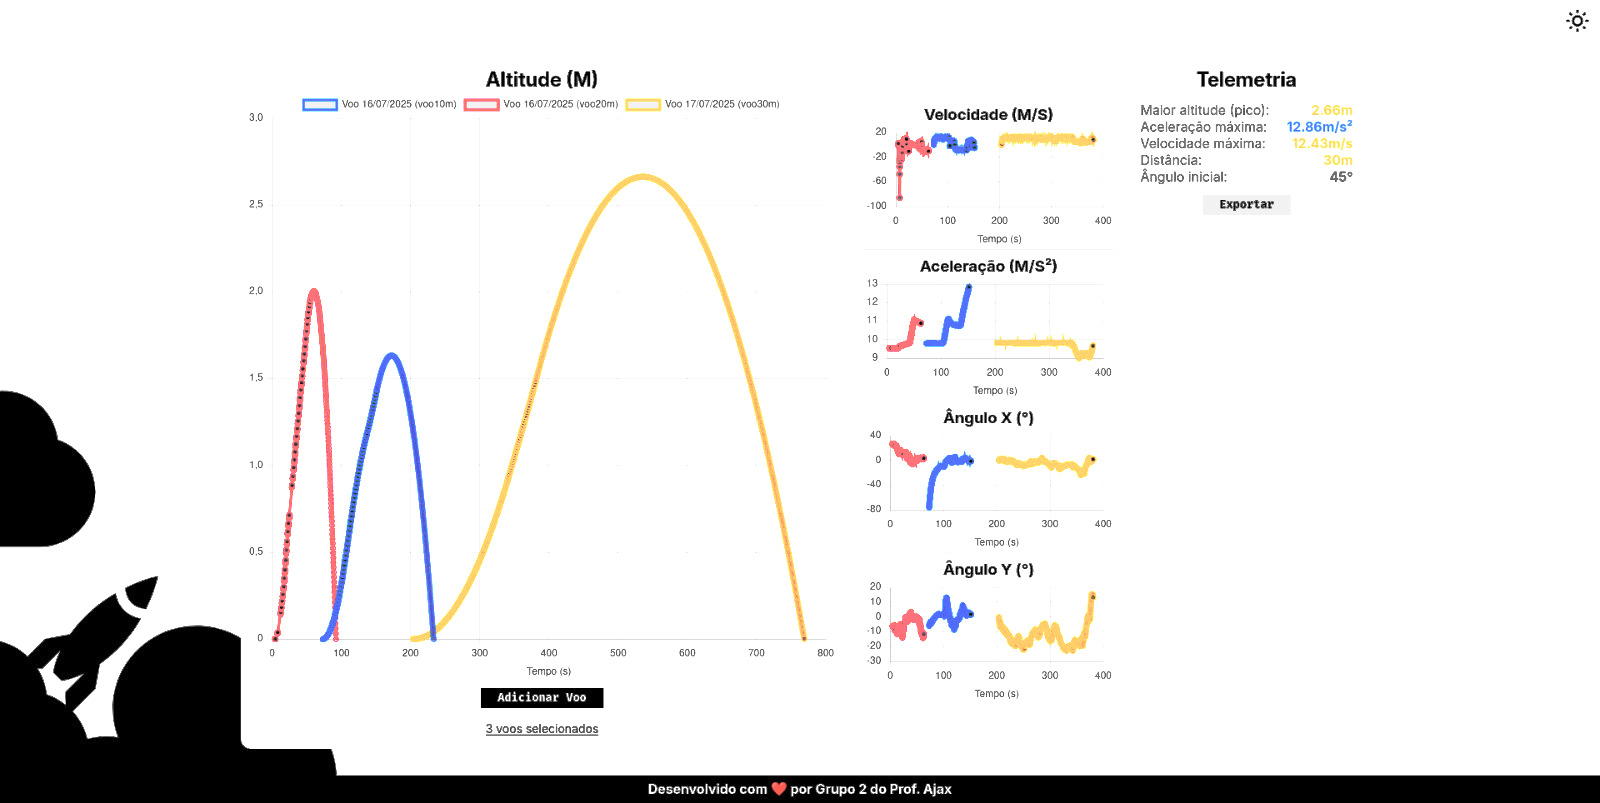
\includegraphics[width=\linewidth,keepaspectratio]{figuras/software/graficos.jpeg}
\caption{Gráficos de desempenho dos voos.}
\label{fig_graficos}
\end{figure}

\end{landscape}

\end{samepage}
% \subsection{Plano de testes}

\begin{figure}[H]
    \centering
\begin{longtable}{|p{0.2\textwidth}|p{0.7\textwidth}|}
\hline
\multicolumn{2}{|l|}{\textbf{CT01 - Importação de Arquivo JSON Válido}} \\
\hline
\textbf{Tipo} & Teste de sistema \\
\hline
\textbf{Objetivo} & Verificar se o sistema é capaz de importar corretamente um arquivo JSON com dados válidos. \\
\hline
\textbf{Pré-condições} & O sistema deve estar iniciado. Deve haver um arquivo "database.json" com dados completos e corretos no formato esperado.  \\
\hline
\textbf{Procedimentos} & Abrir o sistema. Acessar a funcionalidade "Importar Dados". Selecionar o arquivo "database.json". Confirmar importação. \\
\hline
\textbf{Resultado esperado} & O sistema exibe mensagem de sucesso. Os dados são carregados na interface. Nenhum erro é exibido. \\
\hline
\textbf{Especificação do Reparo} & Verificar se o parser JSON está tratando corretamente os campos esperados. Validar se o caminho de acesso ao arquivo está correto. Corrigir o tratamento de erros silenciosos na importação. \\
\hline
\textbf{Resultado Após Reparo} & O sistema importa corretamente arquivos válidos e exibe os dados esperados. Teste é reexecutado e aprovado. \\
\hline
\end{longtable}
\caption{Caso de Teste 01 - Importação de Arquivo JSON Válido}
\label{fig_ct01_importacao_json_valido}
\end{figure}

\begin{figure}[H]
    \centering
\begin{longtable}{|p{0.2\textwidth}|p{0.7\textwidth}|}
\hline
\multicolumn{2}{|l|}{\textbf{CT02 - Importação de JSON com campos ausentes}} \\
\hline
\textbf{Tipo} & Sistema \\
\hline
\textbf{Objetivo} & Verificar o comportamento do sistema ao importar registros incompletos. \\
\hline
\textbf{Pré-condições} & Arquivo "dados\_incompletos.json" com campos obrigatórios ausentes. \\
\hline
\textbf{Procedimentos} & Acessar "Importar Dados". Selecionar "dados\_incompletos.json". Confirmar importação. \\
\hline
\textbf{Resultado esperado} & Sistema identifica e ignora os registros inválidos. \\
\hline
\textbf{Especificação do Reparo} & Adicionar validação de campos obrigatórios durante o parsing. \\
\hline
\textbf{Resultado após Reparo} & Registros incompletos tratados corretamente. \\
\hline
\end{longtable}
\caption{Caso de Teste 02 - Importação de JSON com campos ausentes}
\label{fig_ct02_importacao_json_campos_ausentes}
\end{figure}

\begin{figure}[H]
    \centering
\begin{longtable}{|p{0.2\textwidth}|p{0.7\textwidth}|}
\hline
\multicolumn{2}{|l|}{\textbf{CT03 - Importação de formato inválido}} \\
\hline
\textbf{Tipo} & Sistema \\
\hline
\textbf{Objetivo} & Garantir que o sistema rejeita arquivos com extensão JSON mas conteúdo inválido (ex: JSON). \\
\hline
\textbf{Pré-condições} & Arquivo "dados\_errados.json" contendo dados JSON. \\
\hline
\textbf{Procedimentos} & Tentar importar "dados\_errados.json". \\
\hline
\textbf{Resultado esperado} & Mensagem de erro de formato exibida. \\
\hline
\textbf{Especificação do Reparo} & Validar estrutura JSON no momento da importação. \\
\hline
\textbf{Resultado após Reparo} & Sistema rejeita corretamente arquivos malformados. \\
\hline
\end{longtable}
\caption{Caso de Teste 03 - Importação de formato inválido}
\label{fig_ct03_importacao_formato_invalido}
\end{figure}

\begin{figure}[H]
    \centering
\begin{longtable}{|p{0.2\textwidth}|p{0.7\textwidth}|}
\hline
\multicolumn{2}{|l|}{\textbf{CT04 - Exportação de Dados para JSON}} \\
\hline
\textbf{Tipo} & Sistema \\
\hline
\textbf{Objetivo} & Garantir que os dados processados sejam exportados corretamente para JSON. \\
\hline
\textbf{Pré-condições} & Dados processados e disponíveis na interface. \\
\hline
\textbf{Procedimentos} & Clicar em "Exportar Dados".  Selecionar "Formato JSON".  Salvar arquivo.  \\
\hline
\textbf{Resultado esperado} & Arquivo JSON é gerado com os dados exibidos. \\
\hline
\textbf{Especificação do Reparo} & Corrigir função de exportação e formatação de colunas. \\
\hline
\textbf{Resultado após Reparo} & Arquivo JSON correto é gerado. \\
\hline
\end{longtable}
\caption{Caso de Teste 04 - Exportação de Dados para JSON}
\label{fig_ct05_exportacao_dados_csv}
\end{figure}

\begin{figure}[H]
    \centering
\begin{longtable}{|p{0.2\textwidth}|p{0.7\textwidth}|}
\hline
\multicolumn{2}{|l|}{\textbf{CT05 – Responsividade da Interface}} \\
\hline
\textbf{Tipo} & Sistema \\
\hline
\textbf{Objetivo} & Verificar o comportamento da interface em diferentes resoluções da tela. \\
\hline
\textbf{Pré-condições} & Sistema em execução. \\
\hline
\textbf{Procedimentos} & Acessar a aplicação em diferentes tamanhos de tela. Navegar pelas funcionalidades. \\
\hline
\textbf{Resultado esperado} & Componentes se ajustam corretamente, sem sobreposições ou corte. \\
\hline
\textbf{Especificação do Reparo} & Ajustar responsividade. \\
\hline
\textbf{Resultado após Reparo} & Interface se adapta corretamente a todas as resoluções testadas. \\
\hline
\end{longtable}
\caption{Caso de Teste 05 - Responsividade da Interface}
\label{fig_ct06_responsividade_interface}
\end{figure}

\begin{figure}[H]
    \centering
\begin{longtable}{|p{0.2\textwidth}|p{0.7\textwidth}|}
\hline
\multicolumn{2}{|l|}{\textbf{CT06 - Validação dos sensores no lançamento do foguete}} \\
\hline
\textbf{Tipo} & Sistema \\
\hline
\textbf{Objetivo} & Verificar se os dados coletados pelos sensores (pressão, ângulo, massa) estão sendo corretamente lidos e registrados no início do lançamento. \\
\hline
\textbf{Pré-condições} & Sistema embarcado ligado.  Foguete pronto para lançamento.  Todos os sensores conectados corretamente. \\
\hline
\textbf{Procedimentos} & Ligar o sistema de aquisição de dados.  Acionar o lançamento do foguete.  Verificar os dados registrados pelos sensores na interface de análise. \\
\hline
\textbf{Resultado Esperado} & Os dados de pressão, ângulo e massa devem ser capturados corretamente, sem valores nulos ou inconsistentes, e armazenados no JSON gerado. \\
\hline
\textbf{Especificação do Reparo} & Verificar conexões físicas dos sensores, calibrar sensores com valores reais, corrigir erros de leitura no firmware. \\
\hline
\textbf{Resultado Após Reparo} & Os sensores coletam os dados de forma correta e os valores são exibidos e armazenados conforme esperado. \\
\hline
\end{longtable}
\caption{Caso de Teste 06 - Validação dos sensores no lançamento do foguete}
\label{fig_ct07_validacao_sensores_lancamento_foguete}
\end{figure}

\begin{figure}[H]
    \centering
\begin{longtable}{|p{0.2\textwidth}|p{0.7\textwidth}|}
\hline
\multicolumn{2}{|l|}{\textbf{CT07 - Funcionamento do mecanismo de lançamento}} \\
\hline
\textbf{Tipo} & Sistema \\
\hline
\textbf{Objetivo} & Verificar o funcionamento do mecanismo de lançamento. \\
\hline
\textbf{Pré-condições} & Sistema embarcado ligado.  Foguete carregado com água e pressurizado. \\
\hline
\textbf{Procedimentos} & Acionar o sistema de lançamento via interface.  Observar o funcionamento do atuador eletromecânico. \\
\hline
\textbf{Resultado Esperado} & O foguete deve ser lançado automaticamente após o comando, sem falhas mecânicas ou atraso. \\
\hline
\textbf{Especificação do Reparo} & Verificar fiação, tensão e código do acionamento do atuador. \\
\hline
\textbf{Resultado Após Reparo} & Atuador funciona corretamente e o foguete é lançado de forma imediata e estável. \\
\hline
\end{longtable}
\caption{Caso de Teste 07 - Funcionamento do mecanismo de lançamento}
\label{fig_ct08_funcionamento_mecanismo_lancamento}
\end{figure}

\subsection*{Testes de Integração}

\begin{figure}[H]
    \centering
\begin{longtable}{|p{0.2\textwidth}|p{0.7\textwidth}|}
\hline
\multicolumn{2}{|l|}{\textbf{CT08 - Geração dos gráficos}} \\
\hline
\textbf{Tipo} & Integração \\
\hline
\textbf{Objetivo} & Verificar se o sistema gera corretamente o gráfico de altitude após a importação dos dados. \\
\hline
\textbf{Pré-condições} & Dados válidos já importados. \\
\hline
\textbf{Procedimentos} & Acessar a interface de visualização de gráficos. \\
\hline
\textbf{Resultado Esperado} & Gráfico exibido com dados coerentes. \\
\hline
\textbf{Especificação do Reparo} & Ajustar lógica de plotagem ou eixos do gráfico. \\
\hline
\textbf{Resultado após Reparo} & Gráfico é exibido corretamente. \\
\hline
\end{longtable}
\caption{Caso de Teste 08 - Geração dos gráficos}
\label{fig_ct04_geracao_graficos}
\end{figure}

\begin{figure}[H]
    \centering
\begin{longtable}{|p{0.2\textwidth}|p{0.7\textwidth}|}
\hline
\multicolumn{2}{|l|}{\textbf{CT09 - Integração entre ESP32 e Sensores}} \\
\hline
\textbf{Tipo} & Integração \\
\hline
\textbf{Objetivo} & Verificar se os sensores (pressão, ângulo, massa) estão integrados corretamente ao ESP32 e geram dados coerentes. \\
\hline
\textbf{Pré-condições} & Firmware embarcado finalizado.  Todos os sensores ligados ao ESP32. \\
\hline
\textbf{Procedimentos} & Iniciar sistema embarcado.  Coletar dados em tempo real dos sensores.  Verificar se os dados são salvos e transmitidos corretamente. \\
\hline
\textbf{Resultado esperado} & Leituras coerentes e disponíveis para transmissão e armazenamento. \\
\hline
\textbf{Especificação do Reparo} & Verificar drivers de sensores, conexões físicas e timing de leitura. \\
\hline
\textbf{Resultado após Reparo} & Sistema lê e integra dados sem falhas ou atrasos. \\
\hline
\end{longtable}
\caption{Caso de Teste 09 - Integração entre ESP32 e Sensores}
\label{fig_ct24_integracao_esp32_sensores}
\end{figure}

\begin{figure}[H]
    \centering
\begin{longtable}{|p{0.2\textwidth}|p{0.7\textwidth}|}
\hline
\multicolumn{2}{|l|}{\textbf{CT10 - Integração Energética – Estabilidade no Sistema Completo}} \\
\hline
\textbf{Tipo} & Integração \\
\hline
\textbf{Objetivo} & Verificar se a fonte de energia dimensionada suporta o consumo de todos os componentes ao mesmo tempo. \\
\hline
\textbf{Pré-condições} & Sistema montado com todos os sensores e atuadores ativos.  Fonte de energia de 3,3 V e corrente maior que 300\,mA. \\
\hline
\textbf{Procedimentos} & Ligar todos os módulos simultaneamente (ex: pressão, atuadores, display, etc.).  Observar estabilidade de tensão e corrente durante 30 segundos.  Verificar se não ocorrem quedas ou falhas. \\
\hline
\textbf{Resultado esperado} & Tensão estável ($\pm 6\%$) e corrente $\le$ capacidade máxima ($300$)mA. \\
\hline
\textbf{Especificação do Reparo} & Substituir a fonte por uma de maior capacidade ou revisar fiação. \\
\hline
\textbf{Resultado após Reparo} & Sistema opera sem oscilações ou falhas de alimentação. \\
\hline
\end{longtable}
\caption{Caso de Teste 10 - Integração Energética – Estabilidade no Sistema Completo}
\label{fig_ct26_integracao_energetica_estabilidade_sistema_completo}
\end{figure}

\subsection*{Testes de Unidade}

\begin{figure}[H]
    \centering
\begin{longtable}{|p{0.2\textwidth}|p{0.7\textwidth}|}
\hline
\multicolumn{2}{|l|}{\textbf{CT11 - Parser de JSON Válido}} \\
\hline
\textbf{Tipo} & Unidade \\
\hline
\textbf{Objetivo} & Verificar leitura de JSON com dados completos. \\
\hline
\textbf{Pré-condições} & Função de parser implementada e disponível no ambiente de desenvolvimento.  Arquivo de teste válido com dados completos. \\
\hline
\textbf{Procedimentos} & Rodar função de parser diretamente com arquivo de teste válido.  Verificar se estrutura retornada está correta. \\
\hline
\textbf{Resultado esperado} & Dados carregados na memória, sem exceções. \\
\hline
\textbf{Especificação do Reparo} & Revisar lógica de leitura e formatação do JSON.  Corrigir tratamento de exceções ou formatação incorreta. \\
\hline
\textbf{Resultado após Reparo} & Parser reconhece corretamente arquivos válidos e gera a estrutura esperada sem exceções. \\
\hline
\end{longtable}
\caption{Caso de Teste 11 - Parser de JSON Válido}
\label{fig_ct09_parser_json_valido}
\end{figure}

\begin{figure}[H]
    \centering
\begin{longtable}{|p{0.2\textwidth}|p{0.7\textwidth}|}
\hline
\multicolumn{2}{|l|}{\textbf{CT12 - Parser de JSON com Campos Ausentes}} \\
\hline
\textbf{Tipo} & Unidade \\
\hline
\textbf{Objetivo} & Garantir tratamento de dados incompletos. \\
\hline
\textbf{Pré-condições} & Função de parser em funcionamento.  JSON de teste com campos ausentes. \\
\hline
\textbf{Procedimentos} &  Rodar parser com JSON que tenha campos ausentes.  Verificar se registros inválidos são removidos. \\
\hline
\textbf{Resultado esperado} & Retorno apenas dos registros completos. \\
\hline
\textbf{Especificação do Reparo} & Corrigir verificação de campos obrigatórios.  Implementar descartes controlados de registros inválidos. \\
\hline
\textbf{Resultado após Reparo} & Parser filtra registros incompletos sem falhas. \\
\hline
\end{longtable}
\caption{Caso de Teste 12 - Parser de JSON com Campos Ausentes}
\label{fig_ct10_parser_json_campos_ausentes}
\end{figure}

\begin{figure}[H]
    \centering
\begin{longtable}{|p{0.2\textwidth}|p{0.7\textwidth}|}
\hline
\multicolumn{2}{|l|}{\textbf{CT13 - Parser de JSON com Dados Absurdos}} \\
\hline
\textbf{Tipo} & Unidade \\
\hline
\textbf{Objetivo} & Verificar descarte de dados absurdos (ex: altitude negativa). \\
\hline
\textbf{Pré-condições} & Função de validação em funcionamento.  Lista de dados brutos com registros absurdos. \\
\hline
\textbf{Procedimentos} & Rodar função de validação com lista de dados brutos.  Observar se registros absurdos são filtrados. \\
\hline
\textbf{Resultado esperado} & Lista resultante sem registros absurdos. \\
\hline
\textbf{Especificação do Reparo} & Corrigir regra de validação de campos.  Implementar descarte de dados absurdos. \\
\hline
\textbf{Resultado após Reparo} & Função remove corretamente dados absurdos sem impactar o restante. \\
\hline
\end{longtable}
\caption{Caso de Teste 13 - Parser de JSON com Dados Absurdos}
\label{fig_ct27_parser_json_dados_absurdos}
\end{figure}

\begin{figure}[H]
    \centering
\begin{longtable}{|p{0.2\textwidth}|p{0.7\textwidth}|}
\hline
\multicolumn{2}{|l|}{\textbf{CT14 - Aplicação de Filtro de Média Móvel}} \\
\hline
\textbf{Tipo} & Unidade \\
\hline
\textbf{Objetivo} & Verificar aplicação correta de filtro. \\
\hline
\textbf{Pré-condições} & Função de filtro implementada.  Dados de teste com ruído disponíveis.  \\
\hline
\textbf{Procedimentos} & Rodar função de filtro com dados de teste (com ruído).  Comparar saída com valores esperados (média móvel conhecida).  \\
\hline
\textbf{Resultado esperado} & Dados suavizados sem distorção indevida. \\
\hline
\textbf{Especificação do Reparo} & Ajustar janela ou lógica de média móvel.  Corrigir cálculos que gerem resultados errados. \\
\hline
\textbf{Resultado após Reparo} & Filtro suaviza corretamente os dados e remove ruídos. \\
\hline
\end{longtable}
\caption{Caso de Teste 14 - Aplicação de Filtro de Média Móvel}
\label{fig_ct11_filtro_media_movel}
\end{figure}

\begin{figure}[H]
    \centering
\begin{longtable}{|p{0.2\textwidth}|p{0.7\textwidth}|}
\hline
\multicolumn{2}{|l|}{\textbf{CT15 - Exportação de Dados para JSON}} \\
\hline
\textbf{Tipo} & Unidade \\
\hline
\textbf{Objetivo} & Validar formatação e consistência do JSON. \\
\hline
\textbf{Pré-condições} & Função de exportação implementada e em funcionamento.  Dados em memória para exportação. \\
\hline
\textbf{Procedimentos} & Rodar função de exportação com dados em memória.  Abrir JSON e verificar cabeçalhos, formato e integridade dos dados. \\
\hline
\textbf{Resultado esperado} & Arquivo JSON gerado sem erros. \\
\hline
\textbf{Especificação do Reparo} & Corrigir escrita do arquivo JSON (formato e separadores).  Ajustar cabeçalhos e ordem de dados. \\
\hline
\textbf{Resultado após Reparo} & JSON exportado corretamente e sem inconsistências. \\
\hline
\end{longtable}
\caption{Caso de Teste 15 - Exportação de Dados para JSON}
\label{fig_ct12_exportacao_dados_csv}
\end{figure}

\begin{figure}[H]
    \centering
\begin{longtable}{|p{0.2\textwidth}|p{0.7\textwidth}|}
\hline
\multicolumn{2}{|l|}{\textbf{CT16 - Geração de gráfico}} \\
\hline
\textbf{Tipo} & Unidade \\
\hline
\textbf{Objetivo} & Validar coerência visual dos gráficos gerados. \\
\hline
\textbf{Pré-condições} & Função de geração de gráficos implementada.  Dados de teste consistentes.  \\
\hline
\textbf{Procedimentos} & Rodar função de geração de gráficos com dados de teste.  Conferir se gráfico está correto visualmente e numericamente.  \\
\hline
\textbf{Resultado esperado} & Gráfico gerado com dados coerentes e layout adequado. \\
\hline
\textbf{Especificação do Reparo} &  Ajustar lógica de plotagem (eixos e escalas).  Corrigir erros de indexação de dados.  \\
\hline
\textbf{Resultado após Reparo} & Gráficos exibem dados de forma coerente e confiável. \\
\hline
\end{longtable}
\caption{Caso de Teste 16 - Geração de gráfico}
\label{fig_ct13_geracao_grafico}
\end{figure}

\begin{figure}[H]
    \centering
\begin{longtable}{|p{0.2\textwidth}|p{0.7\textwidth}|}
\hline
\multicolumn{2}{|l|}{\textbf{CT17 - Validação do Sensor MPX5700 (Pressão)}} \\
\hline
\textbf{Tipo} & Unidade (hardware/embarcado) \\
\hline
\textbf{Objetivo} & Garantir leitura coerente da pressão durante carregamento. \\
\hline
\textbf{Pré-condições} & Sistema embarcado ligado e calibrado. \\
\hline
\textbf{Procedimentos} &  Pressurizar gradualmente a câmara.  Ler valores do sensor de pressão.  Comparar com medidor externo confiável.  \\
\hline
\textbf{Resultado esperado} & Leituras consistentes, sem desvios bruscos. \\
\hline
\textbf{Especificação do Reparo} & Calibrar sensor ou corrigir conversão no firmware. \\
\hline
\textbf{Resultado após Reparo} & Leituras de pressão confiáveis e coerentes. \\
\hline
\end{longtable}
\caption{Caso de Teste 17 - Validação do Sensor MPX5700 (Pressão)}
\label{fig_ct14_validacao_sensor_mpx5700}
\end{figure}

\begin{figure}[H]
    \centering
\begin{longtable}{|p{0.2\textwidth}|p{0.7\textwidth}|}
\hline
\multicolumn{2}{|l|}{\textbf{CT18 - Validação do Sensor MPU-6500 (Acelerômetro)}} \\
\hline
\textbf{Tipo} & Unidade (hardware/embarcado) \\
\hline
\textbf{Objetivo} & Verificar se a leitura de aceleração está coerente com o movimento. \\
\hline
\textbf{Pré-condições} & Sistema embarcado funcional. \\
\hline
\textbf{Procedimentos} &  Simular movimentos suaves e bruscos do foguete.  Observar leituras de aceleração.  \\
\hline
\textbf{Resultado esperado} & Dados refletem as variações reais de movimento. \\
\hline
\textbf{Especificação do Reparo} & Calibrar sensor e revisar código de leitura. \\
\hline
\textbf{Resultado após Reparo} & Sensor reporta acelerações reais de forma confiável. \\
\hline
\end{longtable}
\caption{Caso de Teste 18 - Validação do Sensor MPU-6500 (Acelerômetro)}
\label{fig_ct15_validacao_sensor_mpu6500}
\end{figure}

\begin{figure}[H]
    \centering
\begin{longtable}{|p{0.2\textwidth}|p{0.7\textwidth}|}
\hline
\multicolumn{2}{|l|}{\textbf{CT19 - Leitura do Sensor de Massa}} \\
\hline
\textbf{Tipo} & Unidade \\
\hline
\textbf{Objetivo} & Garantir leitura correta da massa do foguete antes do lançamento. \\
\hline
\textbf{Pré-condições} &  Sensor de massa calibrado.  Massa real conhecida.  \\
\hline
\textbf{Procedimentos} &  Colocar o foguete com massa conhecida na plataforma.  Ler os dados da célula de carga via firmware.  Comparar leitura com massa real medida em balança.  \\
\hline
\textbf{Resultado esperado} & Erro máximo aceitável ($\pm 10$g). \\
\hline
\textbf{Especificação do Reparo} & Verificar calibração e conexão do sensor. Corrigir leituras incorretas no firmware. \\
\hline
\textbf{Resultado após Reparo} & Leitura de massa consistente com o valor real. \\
\hline
\end{longtable}
\caption{Caso de Teste 19 - Leitura do Sensor de Massa}
\label{fig_ct16_leitura_sensor_massa}
\end{figure}

\begin{figure}[H]
    \centering
\begin{longtable}{|p{0.2\textwidth}|p{0.7\textwidth}|}
\hline
\multicolumn{2}{|l|}{\textbf{CT20 - Validação do Dimensionamento Energético}} \\
\hline
\textbf{Tipo} & Unidade \\
\hline
\textbf{Objetivo} & Verificar se o fornecimento de energia atende ao consumo calculado com margem de segurança. \\
\hline
\textbf{Pré-condições} &  Sistema embarcado montado com todos os sensores e atuadores conectados.  Fonte de alimentação dimensionada.  \\
\hline
\textbf{Procedimentos} &  Ligar o sistema completo.  Monitorar tensão e corrente durante 30 segundos.  Verificar se a tensão permanece estável.  Verificar se a corrente total está dentro da faixa de consumo.  \\
\hline
\textbf{Resultado esperado} & Sistema opera sem quedas de tensão ou falhas de alimentação. \\
\hline
\textbf{Especificação do Reparo} & Substituir fonte de alimentação ou ajustar conexões elétricas. \\
\hline
\textbf{Resultado após Reparo} & Sistema estável durante todo o tempo de operação. \\
\hline
\end{longtable}
\caption{Caso de Teste 20 - Validação do Dimensionamento Energético}
\label{fig_ct17_validacao_dimensionamento_energetico}
\end{figure}

\begin{figure}[H]
    \centering
\begin{longtable}{|p{0.2\textwidth}|p{0.7\textwidth}|}
\hline
\multicolumn{2}{|l|}{\textbf{CT21 - Validação do Atuador - Válvula Solenóide}} \\
\hline
\textbf{Tipo} & Unidade \\
\hline
\textbf{Objetivo} & Verificar se a válvula solenóide abre/fecha corretamente sob comando. \\
\hline
\textbf{Pré-condições} &  Sistema embarcado funcional.  Compressor e pressão dentro do esperado.  \\
\hline
\textbf{Procedimentos} &  Acionar a válvula via relé (comando direto no firmware).  Observar se há liberação/fechamento imediato de ar.  \\
\hline
\textbf{Resultado esperado} & Válvula responde rapidamente ao comando sem falhas. \\
\hline
\textbf{Especificação do Reparo} & Verificar conexões elétricas e integridade do relé. \\
\hline
\textbf{Resultado após Reparo} & Válvula abre/fecha conforme esperado. \\
\hline
\end{longtable}
\caption{Caso de Teste 21 - Validação do Atuador - Válvula Solenóide}
\label{fig_ct18_validacao_atuador_valvula_solenoide}
\end{figure}

\begin{figure}[H]
    \centering
\begin{longtable}{|p{0.2\textwidth}|p{0.7\textwidth}|}
\hline
\multicolumn{2}{|l|}{\textbf{CT22 - Validação do Atuador - Compressor}} \\
\hline
\textbf{Tipo} & Unidade \\
\hline
\textbf{Objetivo} & Verificar funcionamento do compressor 12 V durante a fase de pressurização. \\
\hline
\textbf{Pré-condições} & Sistema montado e conectado ao relé. \\
\hline
\textbf{Procedimentos} &  Enviar comando para ativar compressor.  Observar operação estável e sem superaquecimento.  \\
\hline
\textbf{Resultado esperado} & Compressor enche a câmara e atinge pressão esperada. \\
\hline
\textbf{Especificação do Reparo} & Verificar tensão de alimentação, relé e conexões físicas. \\
\hline
\textbf{Resultado após Reparo} & Compressor opera normalmente sem falhas. \\
\hline
\end{longtable}
\caption{Caso de Teste 22 - Validação do Atuador - Compressor}
\label{fig_ct19_validacao_atuador_compressor}
\end{figure}

\begin{figure}[H]
    \centering
\begin{longtable}{|p{0.2\textwidth}|p{0.7\textwidth}|}
\hline
\multicolumn{2}{|l|}{\textbf{CT23 - Validação do Atuador - Buzzer}} \\
\hline
\textbf{Tipo} & Unidade \\
\hline
\textbf{Objetivo} & Verificar se o buzzer emite contagem regressiva sonora. \\
\hline
\textbf{Pré-condições} & Firmware com contagem regressiva implementada. \\
\hline
\textbf{Procedimentos} &  Acionar comando de contagem regressiva.  Observar sequência de sons de 10 a 0.  \\
\hline
\textbf{Resultado esperado} & Sons nítidos e no tempo correto. \\
\hline
\textbf{Especificação do Reparo} & Verificar ligação do buzzer e ajuste do firmware. \\
\hline
\textbf{Resultado após Reparo} & Contagem sonora clara e funcional. \\
\hline
\end{longtable}
\caption{Caso de Teste 23 - Validação do Atuador - Buzzer}
\label{fig_ct20_validacao_atuador_buzzer}
\end{figure}

\begin{figure}[H]
    \centering
\begin{longtable}{|p{0.2\textwidth}|p{0.7\textwidth}|}
\hline
\multicolumn{2}{|l|}{\textbf{CT24 - Validação da Conectividade LoRa (RFM95W)}} \\
\hline
\textbf{Tipo} & Unidade \\
\hline
\textbf{Objetivo} & Garantir comunicação confiável entre ESP32 da base e do foguete. \\
\hline
\textbf{Pré-condições} & Ambientes de teste prontos (foguete e base). \\
\hline
\textbf{Procedimentos} &  Ligar ambos os dispositivos.  Iniciar transmissão de dados de teste do foguete para a base.  Observar recepção sem perdas significativas.  \\
\hline
\textbf{Resultado esperado} & Dados JSON recebidos sem interrupções relevantes. \\
\hline
\textbf{Especificação do Reparo} & Ajustar parâmetros de transmissão ou antenas. \\
\hline
\textbf{Resultado após Reparo} & Comunicação estável e confiável via LoRa. \\
\hline
\end{longtable}
\caption{Caso de Teste 24 - Validação da Conectividade LoRa (RFM95W)}
\label{fig_ct21_validacao_conectividade_lora}
\end{figure}

\begin{figure}[H]
    \centering
\begin{longtable}{|p{0.2\textwidth}|p{0.7\textwidth}|}
\hline
\multicolumn{2}{|l|}{\textbf{CT25 - Validação do Módulo de Armazenamento MicroSD}} \\
\hline
\textbf{Tipo} & Unidade \\
\hline
\textbf{Objetivo} & Garantir que os dados de voo são salvos corretamente no cartão. \\
\hline
\textbf{Pré-condições} & Sistema do foguete funcional e MicroSD inserido. \\
\hline
\textbf{Procedimentos} &  Iniciar simulação de voo.  Salvar dados de sensores no MicroSD.  Remover cartão e abrir no computador.  \\
\hline
\textbf{Resultado esperado} & Arquivo JSON salvo e legível. \\
\hline
\textbf{Especificação do Reparo} & Verificar comandos de escrita no firmware e integridade do MicroSD. \\
\hline
\textbf{Resultado após Reparo} & Dados salvos corretamente e legíveis. \\
\hline
\end{longtable}
\caption{Caso de Teste 25 - Validação do Módulo de Armazenamento MicroSD}
\label{fig_ct22_validacao_modulo_armazenamento_microsd}
\end{figure}